%!TEX root = labo.tex
\setcounter{chapter}{2}
\chapter{Performance Measurements}

In this lab, the performance and throughput in wireless networks will be investigated. Using tools like \incommand{iperf}, we will record the maximum throughput which can be achieved in wireless networks and have a look at the parameters influencing this throughput. 

\section{Bit Rates}

\begin{exercise}{Basic throughput in \wifi{a}}\label{ex:basicTput}
\label{ex:tput1}
	
	This first exercise will give you an insight into the difference in usable throughput and the available bit rate. To determine the throughput, we will be using a tool called \incommand{iperf}. This is a client-server based tool which sends \ac{tcp} or \ac{udp} traffic and reports the measured throughput. Consult the man pages for the details about this tool. A second tool to be used is \incommand{gnuplot}, in order to plot your results in a graph. More info about \incommand{gnuplot} can be found in \cite{gnuplotHome} and a nice tutorial in \cite{gnuplotTut}. A basic gnuplot script to generate your first plots is provided on the course website. The \incommand{iperf} tool is preinstalled on the wireless nodes, while \incommand{gnuplot} is available on the lab PCs.

	\begin{figure}[h!]
		\begin{center}
			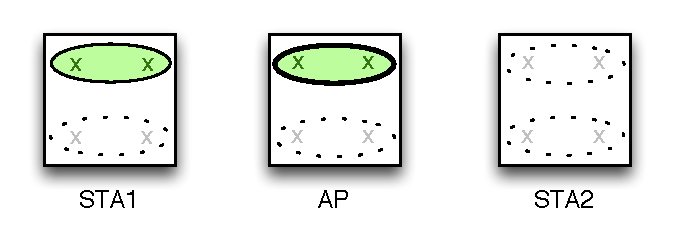
\includegraphics[width=0.5\textwidth]{images/perf1.pdf}
			\caption{Basic throughput setup.} 
			\label{fig:perf1} 
		\end{center}
	\end{figure}
	
	\begin{enumerate}
		\item Start by configuring the setup as shown in figure \ref{fig:perf1}. Use \incommand{fc00:\acs{gid}::3/64} for the \ac{ap} and \incommand{fc00:\acs{gid}::1/64} for \ac{sta}1.
		\item \label{item:rates}\wifi supports various bit rates. Using \incommand{iw list} you can query the supported rates:\newline
		Which rates are supported in \wifi{a}?\newline
		\begin{esolution}
		\end{esolution}
		Which rates are supported in \wifi{b/g}?\newline
		\begin{esolution}
		\end{esolution}
		\item \incommand{iperf} can be used to measure the maximum throughput between two stations. Therefore, a server is started on one end and a client connects on the other end to this server. A connection is set up and as \ac{tcp} tries to maximize the throughput on a connection, an estimate of the maximum throughput on a link can be calculated. When using \incommand{iperf} with the basic parameters, it will perform a 10 seconds test and report the achieved throughput at the client side.
		\item Start a basic \incommand{iperf} session between the \ac{sta} and \ac{ap}, with the \incommand{iperf} server on the \ac{ap}: \newline
		\command{\prompt{AP} iperf -V -s}
		\command{\prompt{STA1} iperf -V -c fc00:\acs{gid}::3 }
		Copy the output of the \incommand{iperf} client:\newline
		\begin{esolution}
		\end{esolution}
	
		\item Now, using \incommand{iperf}, collect the throughput for each available rate and write the results in a file \file{tcp.txt}. On each line, first put the rate followed by a space and then the result in Mbit/s obtained from \incommand{iperf}, e.g. \texttt{54 30} denotes that a 30Mbit/s was measured when using a rate of 54 Mbps. You can change the rate used at the \ac{sta} using \incommand{iw}, e.g. to 54Mbps, as follows:\newline
		\command{\prompt{STA1} iw dev wlan0 set bitrates legacy-5 54}
		You can check the actual used bit rate from the output of \incommand{iwconfig}:\newline
		\command{\prompt{STA1} iwconfig wlan0}
		\remark As we will be repeating the collection of these results in the following exercises, it will be easier to use some bash scripting to speed up this process. 
		A helper script can be found in the file \texttt{iperf-tcp.sh}. Change this script so it loops over the correct bitrates, and use it with the command \incommand{./iperf-tcp.sh fc00:grID::3}.\newline
		This script generates output that can be directly copied to \file{tcp.txt}
		
		
		\item \incommand{iperf} will by default use \ac{tcp} to check the connection, but it is also possible to use a unidirectional \ac{udp} stream. Therefore, one can try to feed more data to the network than the network can support and as such measure how much can be actually delivered. Thus, repeat the previous scenario and collect the maximum achievable throughput using \incommand{iperf} in \ac{udp} mode for each available bit rate. Save these results in the same format as in the previous item in a file \file{udp.txt}.\newline Again, a script called \texttt{udp.sh} is provided that automates this process. The script will try to send a UDP stream that fills the wireless link.\newline
		\command{\prompt{AP} iperf -V -s -u -l 1452}
		\command{\prompt{STA1} ./iperf-udp fc00:grID::3}
		\remark \texttt{-l} is the letter l, not the number one!

		\item Now plot these results using \incommand{gnuplot}. On the course website, a \incommand{gnuplot} script, \texttt{tput1.gnuplot}, is provided to plot the throughput and the relative link usage over the various available rates. The used commands are straightforward and the script is inline commented so should be self-explanatory. Make sure you understand the various commands in the file. The script produces two PDF files which can be viewed with any regular PDF viewer. Place the \texttt{.txt} files you created in the previous steps in the same directory as the \incommand{gnuplot} script. Save the generated files in your lab report as \texttt{L3-1-4-tput.pdf} and \texttt{L3-1-4-usage.pdf}. Add the plots here and shortly discuss what can be observed. Also shortly discuss the difference between \ac{udp} and \ac{tcp}. To generate the PDF files, use:\newline
		\command{gnuplot tput.gnuplot}
		\begin{esolution}
		\end{esolution}
		\end{enumerate}
\end{exercise}

\begin{exercise}{Client to client throughput}
\label{ex:tput2}
	\begin{figure}[h!]
		\begin{center}

			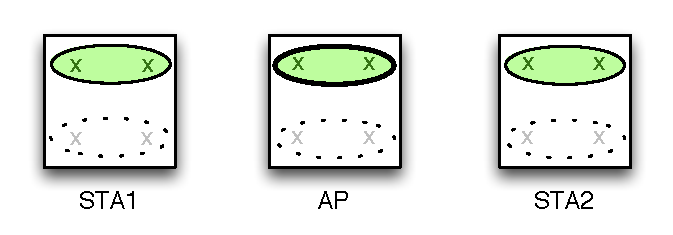
\includegraphics[width=0.5\textwidth]{images/perf2.pdf}
			\caption{Client to client throughput setup.} 
			\label{fig:perf2} 
		\end{center}
	\end{figure}
	
	In the previous exercise, the throughput was measured between a \ac{sta} and the \ac{ap} it was connected to. In this exercise, we are interested in the throughput between two \acp{sta} associated with the same \ac{ap}.
	\begin{enumerate}
		\item Create the test setup as shown in figure \ref{fig:perf2}. Configure \acs{sta}2 with IP address \texttt{fc00:grID::2/64}.
		\item Collect the \ac{tcp} and \ac{udp} throughput measures as in the previous exercise and save them to \file{tcp.txt}\\ and \file{udp.txt}.
		\item Adapt the provided \incommand{gnuplot} script and create graphs for the new measurements. Include them in your report.
		\item Comment on the obtained results and compare the results from this exercise with those from the previous exercise. Explain the difference.\newline
		\begin{esolution}
		\end{esolution} 
	\end{enumerate}
	
\end{exercise}

\section{Network Settings}
\begin{exercise}{\acs{rts}/\acs{cts}}

In lab 2, we enabled the \ac{rts}/\ac{cts} mechanism to show that in \wifi, stations can reserve the medium in order to avoid collisions. In this exercise, we will study the effect of \ac{rts}/\ac{cts} on throughput.

\begin{enumerate}
	\item Enable \ac{rts}/\ac{cts} on all devices.\newline
	\command{\prompt{} iw phy phy0 set rts 1000}
	\item Repeat the iperf tests from \ac{sta}1 to \ac{ap}. Save your logs to \file{tcp.txt}\\ and \file{udp.txt}. Again modify the gnuplot script to create new graphs and include them in your report. To make the comparison more easy, modify the gnuplot script so that you plot both the results from exercise \ref{ex:tput1} and this exercise on the same graph. What do you observe? Why?\newline
	\begin{esolution}
	\end{esolution}

\end{enumerate}

\end{exercise}

\begin{exercise}{Frame length}

	The standard \ac{mtu} for ethernet frames is 1500 bytes. \wifi however allows an \ac{mtu} up to 2274 bytes. In this exercise, you will measure the effect of frame size on throughput.
	
	\begin{enumerate}
		\item Continue from the previous setup, but make sure \ac{rts}/\ac{cts} is turned off on all nodes:\newline
		\command{iw phy phy0 set rts off}
		\item On \ac{sta}1, reset rate control to its default (automatic) value:\newline
		\command{\prompt{\ac{sta}1} iw dev wlan0 set bitrates}
		\item Perform the following tests with 4 different maximum frame sizes: 1500, 1758, 2016 and 2274. The frame size can be controlled by changing the \ac{mtu}. \emph{If you do this, do this on all nodes!}\newline
		\command{ifconfig wlan0 mtu 1758}
		\item For each of the \acp{mtu} mentioned, start with a \ac{tcp} \incommand{iperf} test between \ac{sta} and \ac{ap} as in the previous exercises and make plots for each frame size. Generate a results file called \file{tcp.txt}\\ containing \ac{mtu} and bit rate achieved. The file should have the same format as the ones produced this far, except that the first column now contains your \ac{mtu} setting rather than the link speed.\newline
		\command{\prompt{\ac{sta}1} iperf -V -c fc00:grID::3}
		\item Repeat the tests, now using \ac{udp}. For \incommand{iperf}, use the \incommand {-l}  parameter, followed by the current MTU setting minus 48 (e.g. 1452 if the \ac{mtu} is set to 1500) to generate packets that are large enough to fill the MTU. \stress{This must be done on both client and server!} Save your results to \file{udp.txt}\\.\newline
		\command{\prompt{\ac{sta}1} iperf -V -u -l 1452 -c fc00:grID::3 -b 54M}
    		\item Modify the \incommand{gnuplot} script to generate the same graph as before. Plotting only the throughput versus \ac{mtu} suffices. A relative link usage graph is not required. What do you observe? Why? Be as precise as possible.\newline
		\begin{esolution}
		\end{esolution}	 
	\end{enumerate}
		
\end{exercise}


\section{Packet Size}
\begin{exercise}{IP Fragmenting}

	Changing frame lengths has an effect on the throughput, as you have shown in the previous exercise. However, in that case, traffic was flowing between segments with the  same fragment size. When we consider the default setup of an \ac{ap} which is connected to the Internet, the \ac{wan} link is most likely limited to 1500 bytes per frame and thus IP fragmenting comes into play. In IPv6, fragmenting in intermediate hops is not allowed. The end hosts may, however, fragment the IP packets end-to-end to make sure they fit on the link with the smallest \ac{mtu}. Depending on the original payload length, fragments of various lengths will be created. In this exercise we will have a look at the impact of fragmenting on the overall throughput.
	
	To do so, we will run the \incommand{iperf} server on the third node, which is only connected by wire to the \ac{ap}. Using additional routes, we will create a setup where \ac{sta}1 and \ac{sta}2 communicate via the \ac{ap}. Traffic between \ac{sta}1 and the \ac{ap} will be transmitted on the wireless link, while traffic between the \ac{ap} and \ac{sta}2 will be transmitted on the wired link.
	
	\begin{figure}[h!]
		\begin{center}
			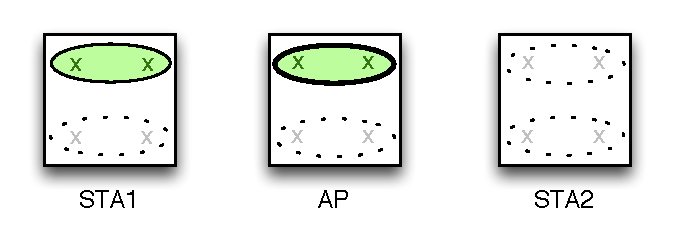
\includegraphics[width=0.5\textwidth]{images/perf1.pdf}
			\caption{Fragmenting setup.} 
			\label{fig:fragmenting} 
		\end{center}
	\end{figure}



	\begin{enumerate}
		\item Start by configuring your setup as shown in figure \ref{fig:fragmenting}. \ac{sta}2 will only be used as \incommand{iperf} server and does not need an active \ac{wnic}.
		\item Set \texttt{fc00:\acs{gid}::3/64} as IP for the \ac{ap} and \texttt{fc00:\acs{gid}::1/64} for \ac{sta}1.
		\item Traffic from \ac{sta}1 to \ac{sta}2 will by default use the wired network. To force a wireless hop, we will add some new routes:\newline
		\command{\prompt{\ac{sta}2} ip route add fc00:\acs{gid}::/64 via <wired IP address of \acs{ap}>}
		\command{\prompt{\ac{sta}1} ip route add <wired IP address of \acs{sta}2>/128 via fc00:\acs{gid}::3}
		\item IPv6 forwarding is by default not enabled on the lab nodes. We must enable it on the \ac{ap} for the setup to work. However, due to a bug, the \ac{ap} will clear its default route when we do this, making it instantly inaccessible over IPv6. Perform the following as a workaround:\newline
		\command{\prompt{\ac{ap}} ip -6 route show | grep default}
		You should get output like this:\newline
		\texttt{default via fe80::225:90ff:fe61:efac dev eth0  proto kernel  metric 1024  expires 1670sec}
		\item Enable IPv6 routing functionality on the \ac{ap}:\newline
		\command{\prompt{\ac{ap}} sysctl -w net.ipv6.conf.all.forwarding=1 \&\& ip route add default via fe80::225:90ff:fe61:efac dev eth0}\newline
		The IP address in that command should be the same as that in the output of the previous step.
		\item Perform a \incommand{traceroute6} from \ac{sta}1 to \ac{sta}2 to check if the routes are set up correctly. Include your traceroute6 output below:\newline
		\command{\prompt{\ac{sta}1} traceroute6 <wired IP address of \acs{sta}2>}\newline
		\begin{esolution}
		\end{esolution}
		\item Now, for each \ac{mtu} (1500, 1758, 2016 and 2274), perform the following:\newline
		\begin{itemize}
			\item Set the \ac{mtu} on the wireless link.
			\item Perform a TCP \incommand{iperf} from \ac{sta}1 to \ac{sta}2.
			\item Perform a UDP \incommand{iperf} from \ac{sta}1 to \ac{sta}2. In each trace, set your frame size to the \ac{mtu} of the wireless link minus 48. Send at a bit rate of 54 Mbps.
		\end{itemize}
		\item The results of your tests should once again be saved to text files like in the previous exercise. Save them to \file{tcp.txt}\\ and \file{udp.txt}\\. Create a throughput graph as in the previous exercise.
		\item You should also make \texttt{.pcap} trace files from these experiments. However, as the link gets fully saturated, the trace file would become very large. Therefore, we will repeat the experiments sending far less traffic. This of course means that you will not see a difference in \incommand{iperf} results. The traces will help you, however, to understand what has happened in the previous exercise.
		\item In order to limit the amount of traffic, we will do the following on \ac{sta}1:
		\begin{itemize}
		\item Set the rate of \texttt{wlan0} to 6 Mbps.
		\item for both TCP and UDP \incommand{iperf}, add the \texttt{-t 2} parameter. This limits the \incommand{iperf} trace to two seconds.
		\item for UDP \incommand{iperf}, omit the \texttt{-b 54M} parameter. This way, \incommand{iperf} will only transmit at 1 Mbps.
		\end{itemize}
		\item Now, do the same \incommand{iperf} tests again, using the above parameters for \incommand{iperf}. For each run, make a \incommand{tcpdump} trace on interface \texttt{wlan0} of the \ac{ap}. Save the traces to \file{tcp.<MTU size>.pcap}\\ and \file{udp.<MTU size>.pcap}\\, respectively.
		\item What do you observe? Distinguish between the behaviour for TCP and UDP. Explain your findings by including your graphs and refering to the trace files you made. Be as precise as possible.\newline
		\begin{esolution}
		
		\end{esolution}
 
	\end{enumerate}	
\end{exercise}